% 2021-04-14
%
% LaTeX file and figures obtained at 2021-04 from Urban
% EPJA LaTeX template files from
% https://mc.manuscriptcentral.com/societyimages/epja/EPJA_templ.zip

\documentclass[epj]{svjour}

\usepackage{amsmath}
\usepackage{graphicx}

\journalname{Eur. Phys. J. A}
\graphicspath{{figures/}}

\begin{document}

\title{Spin-dependent $\boldsymbol{np \rightarrow pn}$ amplitude estimated from
  $\boldsymbol{dp \rightarrow ppn}$}
\author{
  V.V.~Glagolev\inst{1}        \and J.~Hlav\'{a}\v{c}ov\'{a}\inst{2} \and
  M.S.~Khvastunov\inst{1}      \and N.B.~Ladygina\inst{1}            \and
  G.~Martinsk\'{a}\inst{3}     \and J.~Mu\v{s}insk\'{y}\inst{1,3}    \and
  B.~Pastir\v{c}\'{a}k\inst{4} \and N.M.~Piskunov\inst{1}            \and
  T.~Siemiarczuk\inst{5}       \and J.~Urb\'{a}n\inst{3}
}
\institute{
  Joint Institute for Nuclear Research, 141980 Dubna, Russia \and
  Technical University, Park Komensk\'{e}ho 2, SK-04200, Ko\v{s}ice,
  Slovak Republic \and
  University of P.J.\v{S}af\'{a}rik, Jesenn\'{a} 5, SK-04154, Ko\v{s}ice,
  Slovak Republic \and
  Institute of Experimental Physics SAS, Watsonova 47, SK-04353, Ko\v{s}ice,
  Slovak Republic \and
  Institute of Nuclear Studies, ul. Hoza 69, Warsaw, PL-00 681, Poland
}
\date{Received: 25 February 2002 / Revised version: 17 July 2002}
\abstract{
  An estimation of the spin-dependent part of the $np\to pn$ charge exchange
  amplitude was made on the basis of $dp\to (pp)n$ data, taken at 1.67 GeV/c per
  nucleon in a full solid angle arrangement. The $np\to pn$ amplitude turned out
  to be entirely spin-dependent. This result shows new possibilities for
  experiments using polarized deuteron beams and polarized proton targets.
  \PACS{
    {25.10.+s}{Nuclear reactions involving few-nucleon systems} \and
    {25.45.-z}{$^2$H-induced reactions} \and
    {25.45.Kk}{Charge exchange reactions}
  }
}
\maketitle

\section{Introduction}
The task to build up the theory of the nucleon-nucleon scattering, specially for
the region above 1 GeV, is an outstanding issue and therefore new experimental
data are appreciated. A complete determination of spin-dependent nucleon-nucleon
elastic amplitudes requires many measurements. It requires both spin correlation
parameters $A_{NN}$, etc. and spin transfer parameters $K_{NN}$,
etc.~\cite{Bil}. However, in some cases the picture may be simplified. For
example in the case of the investigation of the spin-dependent contribution to
the elementary $np\to pn$ charge exchange reaction, unpolarized deuteron-proton
interactions can be used, where the neutron spin-orbital state is well
established.

The possibility to use the charge exchange reaction on the unpolarized deuteron
for determination of the spin-dependent part of the $np\to pn$ charge exchange
was emphasized partly in the series of works in
\cite{Mig,Pom,Lap,Dean1,Dean2,Bugg}. The effect can be understood qualitatively
in the following way. Two nucleons, bound in the deuteron may be in $^{3}S_{1}$
and $^{3}D_{1}$ ($T=0$) spatial and spin symmetric states; their isospin is
antisymmetric. In charge exchange at 0$^{\circ}$, the transition from
$^{3}S_{1}$ or $^{3}D_{1}$ to a charge symmetric $^{1}S_{0}$ or $^{1}D_{2}$
state of two protons requires spin flip, in order to satisfy the Pauli principle
and ensure an anti-symmetric total wave function. In this way, the
spin-dependent part of the elementary charge exchange amplitude will be
reflected through the probability of the charge exchange process on the
deuteron.

In the general case the nucleon-nucleon amplitude in the centre of mass can be
presented as
\begin{equation}
  \begin{split}
    M=&\ a+b(\vec\sigma \hat n)(\vec\sigma _i \hat n)+
    c[(\vec\sigma \hat n)+(\vec\sigma _i \hat n)]\\&+
    e(\vec\sigma \hat m)(\vec\sigma _i \hat m)+
    f(\vec\sigma \hat l)(\vec\sigma _i \hat l),
  \end{split}
\end{equation}
where the orthonormal basis
\begin{equation}
  \hat l =\frac {\vec k +\vec k^\prime}{|\vec k +\vec k^\prime|},~~
  \hat m =\frac {\vec k -\vec k^\prime}{|\vec k -\vec k^\prime|},~~
  \hat n =\frac {\vec k \times\vec k^\prime}{|\vec k \times\vec k^\prime|}
\end{equation}
introduced in~\cite{Gold} is used. The vectors $\vec k$ and $\vec k^\prime$ are
the initial and final momenta, respectively, $\vec\sigma $ and $\vec\sigma_i$
are the Pauli matrices corresponding to the fast particle and the struck nucleon
from the deuteron, respectively.

In the impulse approximation the $dp$ charge exchange differential cross section
at small momentum transfer $|t|$ is related to the $NN$-amplitudes via
\begin{equation}
  \begin{split}
    \left( \frac{d\sigma }{dt}\right) (pd\rightarrow n(pp))=&\ [1-F_d(t)]\left(
      \frac{d\sigma _1}{dt}\right)\\&+ \Bigl[1-\frac{1}{3}F_d(t)\Bigr]
    \left(\frac{d\sigma _2}{dt}\right),
  \end{split}
\end{equation}
where
\begin{equation}
  \frac{d\sigma _1}{dt}=|a|^2+|c|^2,\quad
  \frac{d\sigma _2}{dt}=|b|^2+|c|^2+|e|^2+|f|^2,
\end{equation}
$F_d (t)$ denotes the deuteron form factor and the coefficients $a,~b,~c,~e$ and
$f$ refer to spin invariants of the elementary charge exchange amplitude eq.~(1)
\cite{Dean1,Ala}.

In this paper we consider the case, when the scattering angle $\theta$ is very
small, close to zero. Under such kinematical conditions one obtains
\begin{equation}
  b=e \qquad \rm{and} \qquad c=0
\end{equation}
and for the elementary cross section a simple expression can be written,
\begin{equation}
  \frac{d\sigma _1}{dt}=|a|^2, \qquad
  \frac{d\sigma _2}{dt}=2|b|^2+|f|^2\ .
\end{equation}
The amplitude $a$ is spin-independent, and $b$ and $f$ are spin-dependent.

At momentum transfer $\vert t \vert\sim 0$, when $F_d (0)$ = 1, eq.~(3) reduces
to:
\begin{equation}
  \frac{d\sigma }{dt}(pd\rightarrow n(pp))=\frac 23\frac{d\sigma _2}{%
    dt}(np\rightarrow pn).
\end{equation}
Thus, the $dp$-charge exchange differential cross section is fully determined by
spin-dependent parts of elementary $np\to pn$ amplitude.

During recent years considerable progress has been achieved in solving the
problem of construction of the scattering matrix. In the intervening period a
substantial amount of new $np$ data has been accumulated. Nowadays the $pp$
analysis is extended up to a laboratory kinetic energy of 2.5 GeV; the $np$
analysis was truncated at 1.3~GeV. While the situation in the complete
reconstruction of the $pp$ scattering amplitude in the region above 1 GeV is
already satisfactory, the same cannot be stated for $np$ scattering \cite{Arn}.

The aim of the present study was the extraction of information on the elementary
process $np\to pn$. The existing data on that reaction are still very scanty and
concern mainly the $d\sigma/dt$ distribution. As a consequence of the definite
isotopic spin of the two protons, the study of the $dp\to (pp)n$ reaction in the
region of the symmetric spatial part of their wave function may give information
on the spin structure of the elementary amplitude. A study of the
deuteron-proton charge exchange differential cross section $d\sigma/dt$ allows
one to estimate the spin-dependent contribution to the $np\to pn$ reaction
amplitude. Such experimental data do not yet exist. Acceleration of deuterium
beams allows to use them for the determination of the spin-dependent part of
elementary $np\to pn$ charge exchange process in a wide region of energy.

\section{Experiment}
The experimental data were taken with the JINR 1 m hydrogen bubble chamber in a
full solid angle geometry and at a incident deuteron momentum of 3.35 GeV/c. The
use of nuclear beams impinging on a fixed proton target makes all the fragments
of the incoming nuclei fast in the laboratory frame, and thus they can be
detected, well measured and identified practically without losses. On the other
hand, almost all losses, due to the chamber threshold momenta, are concentrated
in the elastic channel. These conditions allow one to study reactions containing
not more than one neutral particle in an exclusive approach. A more detailed
description of the experimental set-up and the processing chain can be found
in~\cite{hbc}.

The recorded pictures were scanned twice for all \linebreak
topologies. Measurements on three projections were used for geometrical
reconstruction and subsequent kinematical analysis of events, if an event failed
on any of the processing steps, all four existing projections were
remeasured. The geometrical reconstruction and the kinematical analysis were
carried out using an appropriate version of the CERN program package based on
the HYDRA library~\cite{hyd}. The ionization of charged secondary particles were
estimated visually. The complete data summary tape contains 237413 events of
$dp$ interactions. A sample of 102757 events fitting the reaction $dp\to ppn$
was collected. The studied events of the $dp\to ppn$ reaction could be divided
in a natural way into two channels:
\begin{enumerate}
\item the charge retention channel, where the proton is the fastest secondary
  particle with respect to the deuteron rest frame, and
\item the charge exchange channel, where the neutron is the fastest secondary
  particle with respect to the deuteron rest frame.
\end{enumerate}
As a result 85239 events are attributed to the charge retention channel and
17518 events corresponding to the charge exchange reaction. The separation of
these two channels is illustrated in fig. 1, showing the distribution of the
four momentum transfer squared~$t$, between target proton and secondary neutron
in the laboratory frame. A quantity defined this way does not depend on the
final proton state, whether it is a spectator or participant (indifferent to the
proton interferency).

The first attempt to determine the contribution of the spin-dependent amplitude
of the $np\to pn$ elementary charge exchange from the differential cross section
of the $dp\to (pp)n$ reaction \cite{Ala}, using the available $pp$ and $np$
scattering data, was carried out in the intial stage of the experiment on a
relatively small part of the processed events. The $pp$ and $np$ scattering data
were ambiguous, the statistics poor and correspondingly the obtained estimate
was indefinite, though it dropped a hint to the enhanced role of the
spin-dependent amplitude in the $np\to pn$ charge exchange.

Using the final statistics of over $10^{5}$ events of the $dp\to ppn$ reaction,
we came back to this problem for two reasons:
\begin{enumerate}
\item To make a direct estimate of the $dp\to (pp)n$ differential cross section
  at $t=0$ on the basis of the Dean formalism \cite{Dean1}.
\item To estimate the possibilities and limitations of a prepared counter
  experiment \cite{Baz}.
\end{enumerate}

In the study of high-energy nuclear reactions, the coordinate system in which
the nucleus is at rest is customarily used. For that reason all the physical
quantities given below are in the deuteron rest frame if not stated otherwise.

\begin{figure}
  \centering
  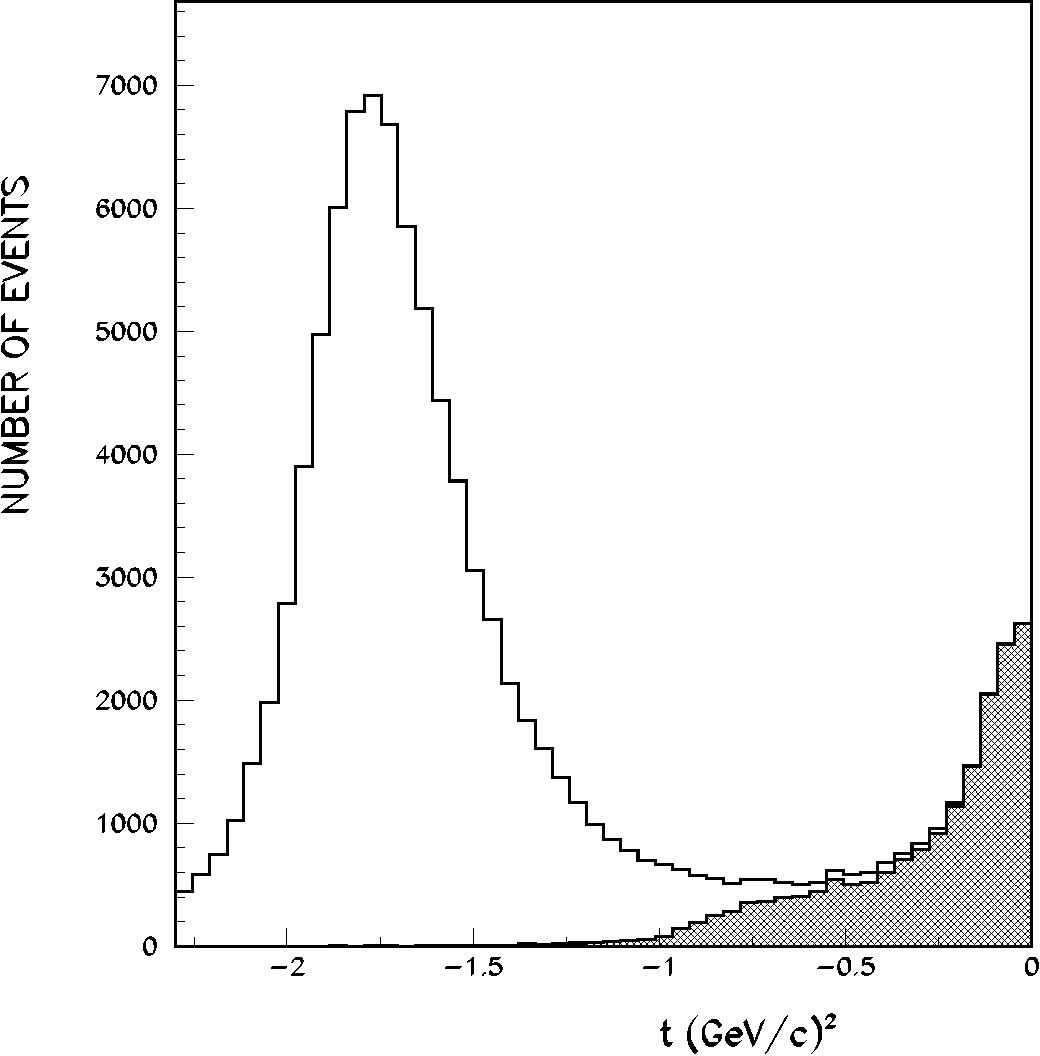
\includegraphics[width=0.82\columnwidth]{fig1.pdf}
  \caption{Distribution of four momentum transfer squared from the target proton
    to the neutron for the $dp\to ppn$ events (dark shaded area: charge exchange
    channel, white area: charge retention channel).}
\end{figure}

\section{Results and discussion}
In order to extract the spin-dependent part of the $np\to pn$ amplitude from the
$dp\to (pp)n$ charge exchange data applying eq. (7), at least the two following
conditions have to be satisfied:
\begin{enumerate}
\item the momentum transfer of the quasielastic $np$ scattering is small,
\item the intrinsic momenta $(q)$ of the nucleons in the \linebreak deuteron are
  small.
\end{enumerate}

The second condition means $S$-wave dominance in the deuteron wave function,
which is shown in fig. 2, where the $S$ wave probability distribution is plotted
as a function of the nucleon intrinsic momentum. In the region below $q$ = 0.07
GeV/c this probability practically does not depend on the nucleon intrinsic
momentum.

Both the above mentioned conditions can be fulfilled simultaneously, if one
selects events in the laboratory \linebreak frame containing two fast protons at
small production angle relative to the incoming deuteron momentum and with
momenta close to half that of the deuteron. We would like to stress, that this
task can be realized successfuly using accelerated deuteron beams. In the case
of a deuteron target the two protons are too slow to be detected and the
reaction cannot be identified. All dedicated charge exchange experiments on a
deuteron so far have been carried out with proton beams.

In addition to the above mentioned, as follows from eq.~(2), to address the
question of the spin-dependent contribution to the $np\to pn$ amplitude, one has
to turn to the data on the differential cross section at $t=0$. Such kind of
data do exist \cite{Fri,She}. They have been obtained at Brookhaven \cite{Fri}
for the region of 1--8 GeV and can be reasonably approximated by $1/p^2$, where
$p$ is the momentum of the incoming neutron. These data imply at $t=0$
$d\sigma/dt$ = (36.9 $\pm$ 3.0) mb/(GeV/c)$^2$ at 1.67 GeV/c. The quoted value
is in good agreement with that obtained from the $np\to pn$ experimental data
\cite{She} at 1.729 GeV/c, fitted by a sum of two exponentials $d\sigma/dt$ =
(36.5 $\pm$ 1.4) mb/(GeV/c)$^2$ (without systematical uncertainties). A similar
behavior of the differential cross section $d\sigma/dt$ at $t=0$ has been
observed below our energies, a peak is present at $u\to 0$ \cite{Bon}.

\begin{figure}
  \centering
  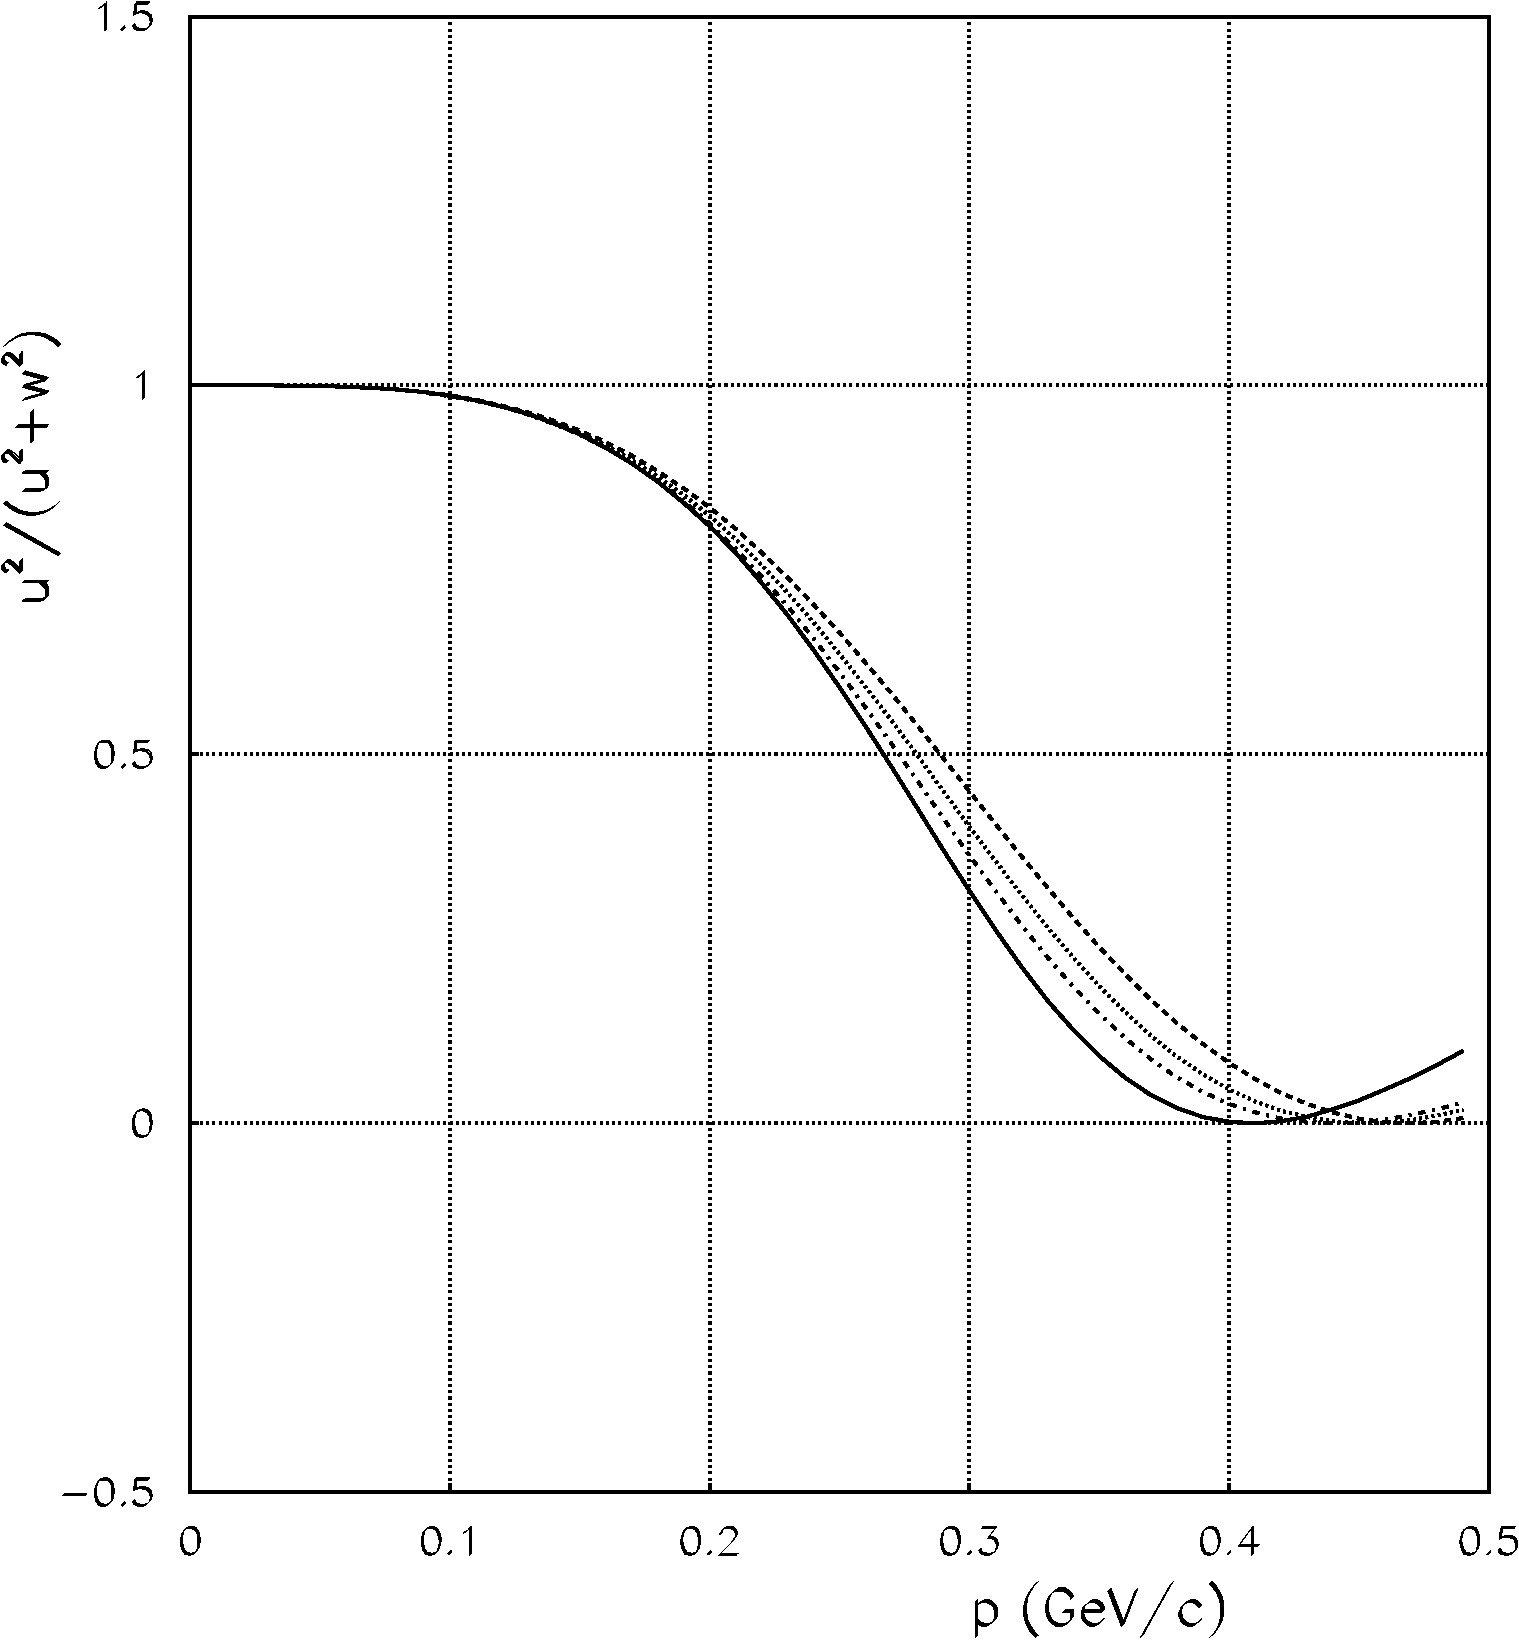
\includegraphics[width=0.95\columnwidth]{fig2.pdf}
  \caption{The $S$-wave probability as a function of the nucleon Fermi momentum.
    Full line: Paris; dashed line: Bonn A; dotted line: Bonn B; dash-dotted
    line: Bonn C wave function.}
\end{figure}

The task is to compare the differential cross section of the charge exchange on
the deuteron, obtained in our experiment at $t=0$ with that for the $np\to pn$
at the corresponding beam energy.

For a reasonable approximation of $d\sigma/dt$ to $t=0$, it is inevitable to
select a region of production angles, excluding the high momentum tails of the
nucleon intrinsic motion and also those regions of momentum transfer, where more
complicated mechanisms than quasi-elastic scattering can come into play. The
changes of the differential cross section at four different values of the two
proton selection angles are illustrated in fig. 3. With the increase of the
angle the character of the $d\sigma/dt$ distribution at small $\vert t \vert$
remains unchanged, while at larger $\vert t \vert$ the contribution increases.

An estimation of the production angle $\theta$ can be obtained, using the
experimental and theoretical maxima ($p_f$ = 50 MeV/c) of the Fermi momentum
distribution of the nucleons in the deuteron as a measure of transverse momentum
and the value of $p_0$ = 1.67 GeV/c for the longitudinal momentum per nucleon in
the laboratory frame. It provides the value
$\theta=arctg(p_f/p_0)=1.6^{\circ}$. This requires that the two protons should
be produced within a cone having an opening angle of $\approx$ 3$^{\circ}$.

\begin{figure}
  \centering
  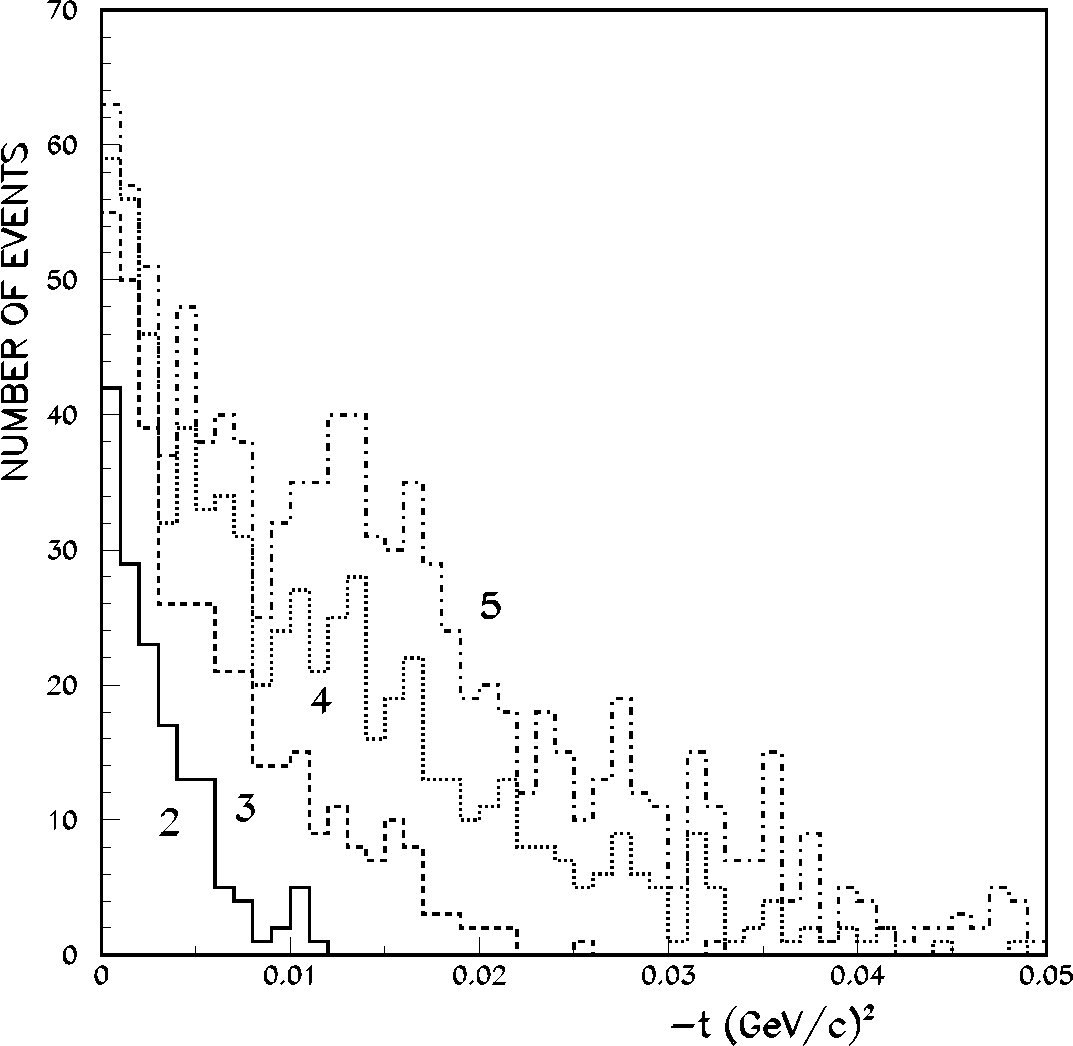
\includegraphics[width=0.88\columnwidth]{fig3.pdf}
  \caption{Distribution of $\vert t \vert$ for the charge exchange channel with
    the production angles of both protons below 2, 3, 4 and 5 degrees.}
\end{figure}
\begin{figure}
  \centering
  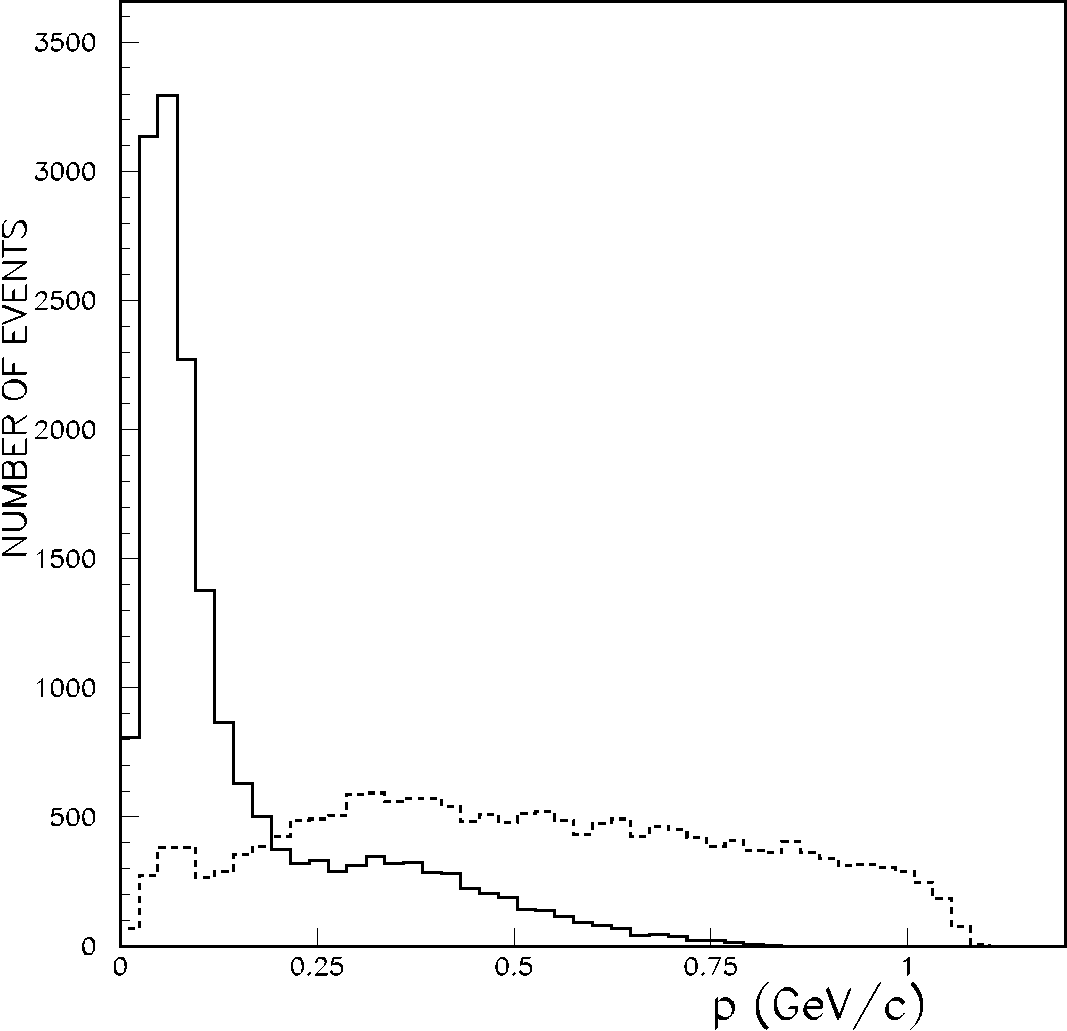
\includegraphics[width=0.88\columnwidth]{fig4.pdf}
  \caption{Momentum distributions of spectator (full line) and scattered protons
    (dashed line) in the deuteron rest frame.}
\end{figure}

In this context we remind the used definitions: the slowest proton in the
deuteron rest frame is referred to as a spectator; the other one we call
scattered. If no cuts are imposed on the proton production angles their momentum
distributions differ significantly as shown in fig.~4.

The spectator proton distribution (full line) follows a curve, typical for the
Fermi momentum distribution in the deuteron. When the above mentioned cut of
3$^\circ$ is applied to the production angles of spectator and scattered proton,
their momentum distributions overlap, as one can see in fig. 5.

\begin{figure}
  \centering
  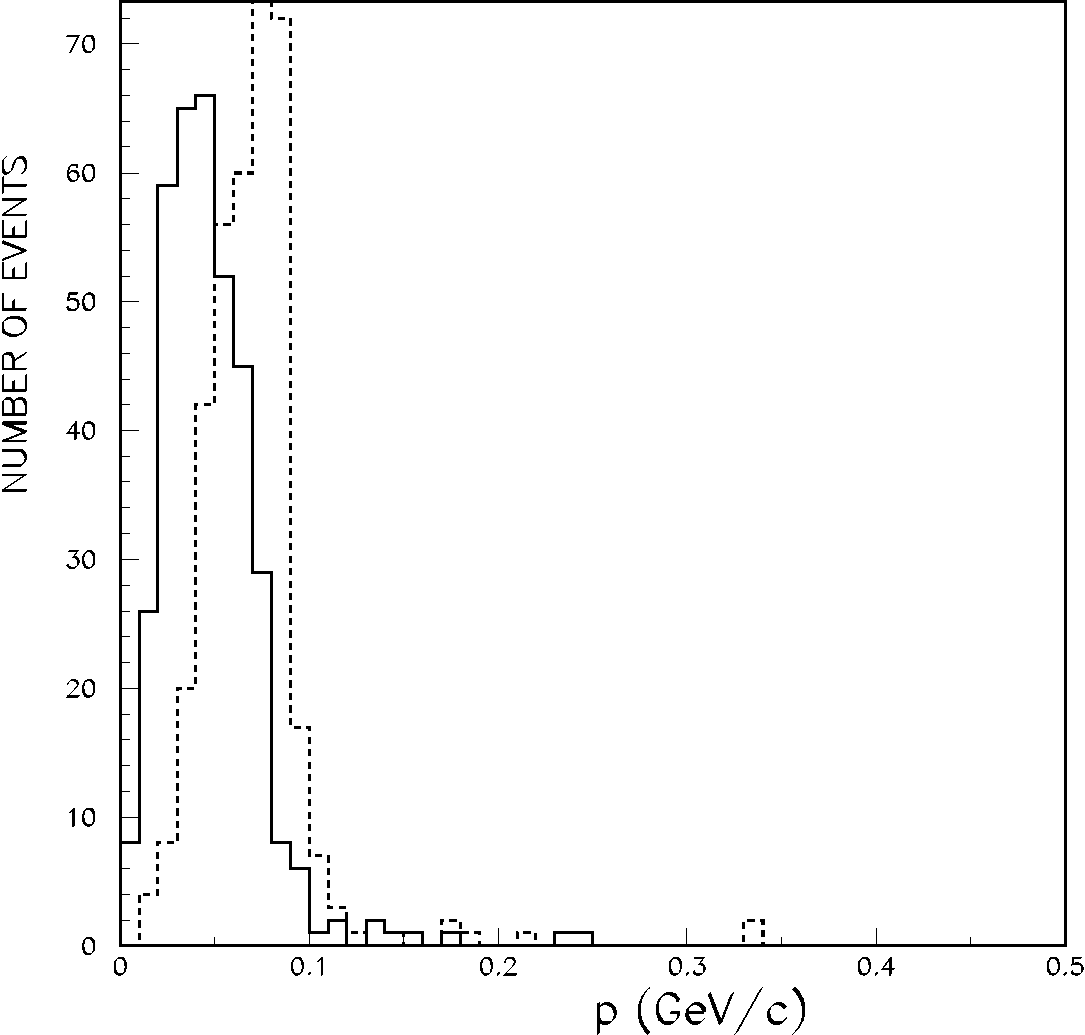
\includegraphics[width=0.92\columnwidth]{fig5.pdf}
  \caption{Momentum distributions of spectator (full line) and scattered protons
    (dashed line) in the deuteron rest frame. The proton production angles in
    the laboratory frame are below 3$^{\circ}$.}
\end{figure}
\begin{figure}
  \centering
  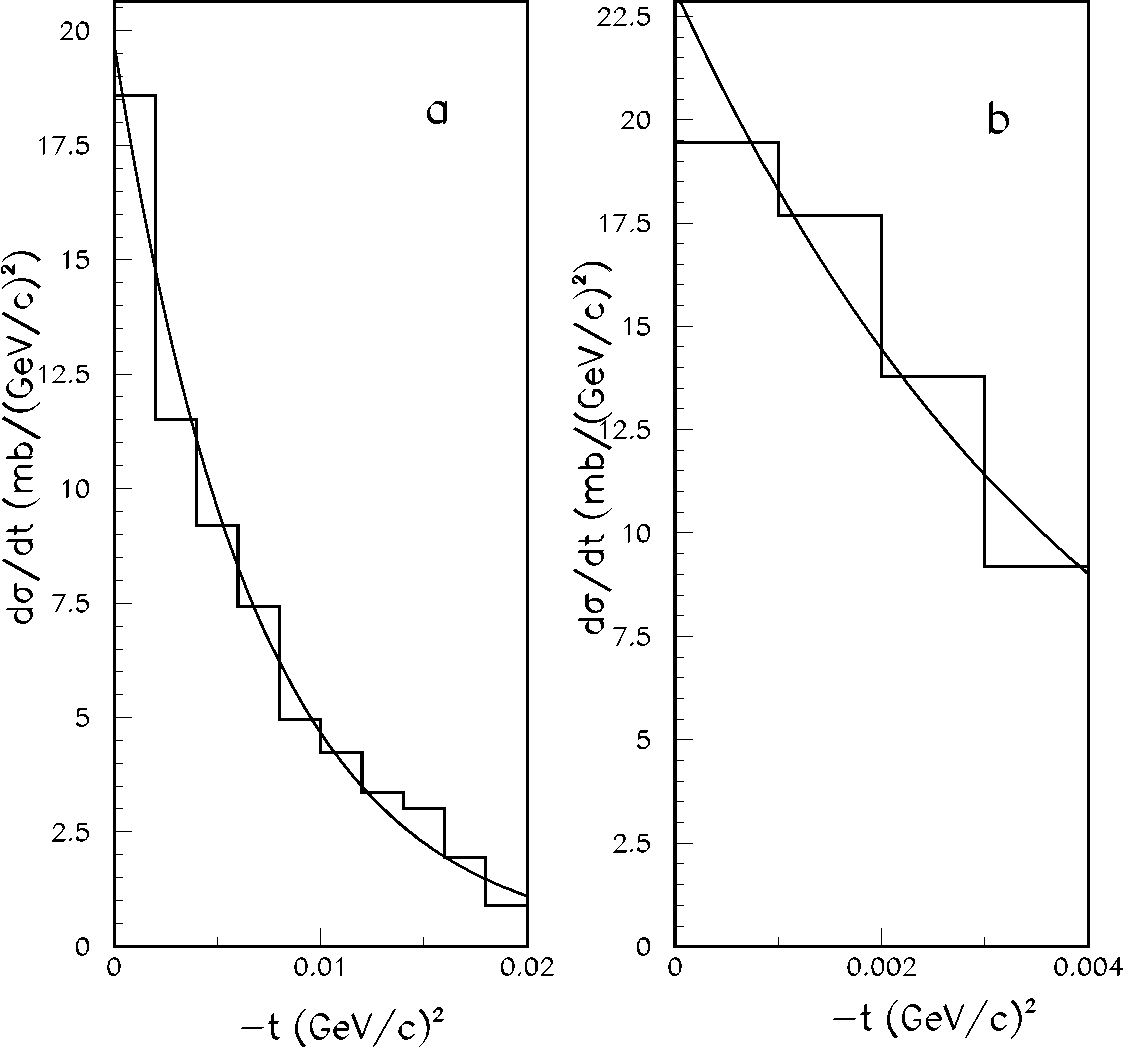
\includegraphics[width=0.92\columnwidth]{fig6.pdf}
  \caption{Differential cross section of the charge exchange reaction in the
    region of small $\vert t \vert$. The production angle of both protons in the
    laboratory frame is in the interval 0--3$^{\circ}$. (b)~shows finer binning
    than~(a).}
\end{figure}

The differential cross section for small values of $\vert t\vert$ is displayed
in fig. 6 together with the curves, corresponding to a fit of $d\sigma/dt$ =
$ae^{bt}$ to the data. The fit gives the following results: $a$ = (19.0 $\pm$
1.1) mb/(GeV/c)$^2$ ($\chi^2$/$ND$~= 4.3/8) for the interval of $\vert t\vert$ =
$\lbrace 0.0\--0.02\rbrace$(GeV/c)$^2$(fig.~6a) and $a$ =
($23.1\genfrac{}{}{0pt}{}{+3.6}{-3.1}$) mb/(GeV/c)$^2$ ($\chi^2$/$ND$ = 1.0/2)
for the interval $\vert t\vert$ = $\lbrace 0.0\--0.004 \rbrace$(GeV/c)$^2$
(fig.~6b).

\begin{figure}
  \centering
  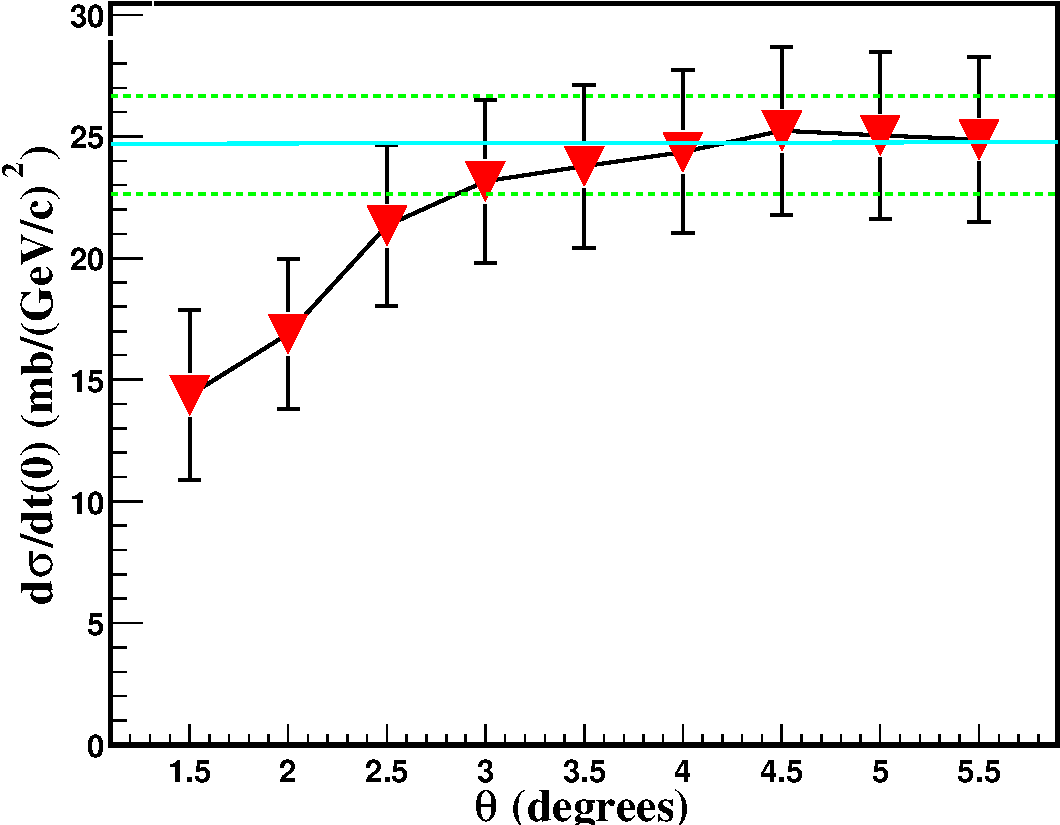
\includegraphics[width=1.00\columnwidth]{fig7.pdf}
  \caption{Differential cross section at $t=0$ when both protons are within a
    cone of opening angle $\theta$. The full line corresponds to 2/3
    $(d\sigma/dt)_{np\to pn}$ at $t=0$, the dashed lines show the
    uncertainties.}
\end{figure}

Figure 7 demonstrates the differential cross section at $t=0$ as a function of
the cut, imposed on the proton production angles. It can be seen in agreement
with eq. (7), that around $\theta$ = 3$^\circ$ the quantity $d\sigma/dt$ at
$t=0$ reaches the level of 2/3 ($d\sigma/dt$) at $t=0$ of the elementary
$np\to pn$ process. For the value of $\theta$ = 3$^\circ$ we get the
contribution of the spin-dependent part to the elementary $np\to pn$ of
$0.94 \pm 0.15$. The obtained contribution of course depends on the systematical
errors of the elementary $np\to pn$ charge exchange cross section~$\approx$~20\%
\cite{She}. In any case the obtained probability is large enough and does not
exclude the amplitude being 100\% spin-dependent in $np\to pn$. The estimate of
the spin-independent part of the amplitude in~\cite{Ala} based on a different
approach and poor statistics (the number of charge exchange events is more than
one order less), did not exclude the nonzero spin-dependent
contribution. Therefore the present results obtained here in a more
straightforward way using eq.~(7) are not in contradiction to our earlier
findings \cite{Ala}. Our experiment allows us to extract only the spin-dependent
part of the $np\to pn$ charge exchange amplitude. Therefore the obtained results
cannot be directly compared with the data taken in polarized proton beam
experiments, \textit{e.g.}~\cite{Rans}. In a future study of the process
$dp\to (pp)n$ using a beam of polarized deuterons one could separate the two
spin-dependent terms in the amplitude of the charge exchange reaction
$np\to pn$, one of which does not conserve while the other conserves the
projection of the nucleon spin onto the direction of momentum at the transition
of the neutron into the proton~\cite{Gla}. The proposed method is applicable in
the energy range up to 10 GeV, where the charge exchange cross section is not
too small. At these energies the phase-shift analysis due to large number of
partial waves is complicated.

\newpage
\section{Conclusion}
The study of the $dp\to (pp)n$ reaction in full solid angle conditions showed,
that the amplitude of the elementary $np\to pn$ charge exchange at 1.67 GeV/c is
practically fully spin-dependent. The obtained result offers new possibilities
to measure the energy dependence of this effect by simultaneous use of both
polarized deuteron beams and polarized proton target.
\\ \\
This work was in part supported by the Grant Agency for Science at the Ministry
of Education of the Slovak Republic (grant No. 1/8041/01).

\begin{thebibliography}{99}
\bibitem{Bil} S.M. Bilenkij, L.I. Lapidus, R.M. Ryndin, Usp. Fiz. Nauk (in
  Russian) {\bf LXXXIV}, 243 (1964)
\bibitem{Mig} A.B. Migdal, J. Exp. Theor. Phys. (in Russian) {\bf 28}, 3 (1955)
\bibitem{Pom} I. Pomeranchuk, Dokl. Akad. Nauk (in Russian) {\bf LXXVIII}, 249
  (1951)
\bibitem{Lap} L.I. Lapidus, J. Exp. Theor. Phys.(in Russian) {\bf 32},1437
  (1957)
\bibitem{Dean1} N.W. Dean, Phys. Rev. {\bf D5}, 1661 (1972)
\bibitem{Dean2} N.W. Dean, Phys. Rev. {\bf D5}, 2832 (1972)
\bibitem{Bugg} D.V. Bugg, C. Wilkin, Nucl. Phys. {\bf A167}, 575 (1987)
\bibitem{Gold} M. Goldberger, K. Watson, Collision Theory, New York, Wiley, 1966
\bibitem{Ala} B.S. Aladashvili et al., Nucl. Phys. {\bf B86}, 461 (1975)
\bibitem{Arn} R.A. Arndt, I.I. Strakovsky, and R.L. Workman, Phys. Rev. {\bf
    C50}, 2731 (1994); R.A. Arndt, I.I. Strakovsky, and R.L. Workman,
  Phys. Rev. {\bf C56}, 3005 (1997); A.de Lesquen et al., Eur. Phys.J. {\bf
    C11}, 69 (1999); C. Lechanoine-Leluc, F. Lehar, P. Winternitz, and
  J. Bystricky, J.Physique {\bf 48}, 985 (1987); R.A. Arndt, I.I. Strakovsky,
  and R.L. Workman, Phys. Rev. {\bf C62}, 034005 (2000)
\bibitem{hbc} B.S. Aladashvili et al., Nucl. Instrum. Methods, {\bf 129}, 109
  (1975); B.S. Aladashvili et al., JINR Commun. 1-7645,Dubna,1973
\bibitem{hyd} V. Framery et al., Hydra Topical Manual TQ Title Package, CERN
  Program Library (1982)
\bibitem{Baz} S.N. Bazylev et al., in Proc. of the Int.Workshop "Relativistic
  nuclear physics from hundreds MeV to TeV", Slovak Republic, Stara Lesna, June
  26-July 1, 2000, p.234
\bibitem{Fri} J.L. Friedes, H. Palevsky, R.L. Stearns, and R.J.Sutter,
  Phys. Rev. Lett. {\bf 15}, 38 (1965)
\bibitem{She} P.F. Shepard, T.J. Devlin, R.E. Mischke, and J. Solomon,
  Phys. Rev. {\bf D10}, 2735 (1974)
\bibitem{Bon} B.E. Bonner et al., Phys. Rev. Lett. {\bf 41}, 1200 (1978)
\bibitem{Rans} R.D. Ransome et al., Phys. Rev. Lett. {\bf 48}, 781 (1982)
\bibitem{Gla} V.V. Glagolev, V.L. Lyuboshitz, V.V. Lyuboshitz, N.M. Piskunov,
  JINR Commun. E1-99-280, Dubna, 1999
\end{thebibliography}

\end{document}
